\documentclass[11pt]{ujarticle}\sloppy
\usepackage{funinfosys}
\usepackage[hyphens]{url}
\usepackage[dvipdfmx]{graphicx}
\author{% 
1021204 西侑亮\\指導教員 : 松原克弥
}		
\course{Informalstion Systems Course}

\title{未来大クラウドシステムにおけるIaC対応によるVM管理の効率化}
\etitle{Implementing a Pluggable IaC Framework on the FUN Educational Cloud System}
\eauthor{Yusuke Nishi}
\abstract{多くの大学において,プログラミング実行環境を提供するクラウドシステムの導入が進んでいる.
クラウドシステムが提供する仮想マシンを用いることで,学生の多様な端末上で統一された実行環境を用意できる.
しかし,学生人数分だけ,仮想マシンの作成や設定をすることは,多くの手間や手順が必要となる.
クラウドシステムをコードで管理する手法であるInfrastructure as Code(IaC)に対応させることで効率的に管理できる.
本研究では,公立はこだて未来大学(以降,未来大)にて使用されているクラウドシステムをIaCに対応させることにより,統一環境を効率よく用意し,講義の効率化を目指す.
}
\keywords{クラウドシステム, IaC, スクレイピング}
\eabstract{
	Nowadays, the number of university is include which use cloud systems for programming develop environment.
	Virtual machines based on cloud systems can be prepared a unified development environment in deferent machines. However, the problem is that many processes are needed to create and configure virtual machines for the number of students. Using of Infrastructure as code (IaC) that the approach of managing Cloud systems by code can be expected to manage efficiently.The study's goal is to improve seminar efficiency by efficiently constructing a unified development environment for the cloud system used at Future University Hakodate (FUN) that is compatible with IaC.
	}

\ekeywords{Cloud System, IaC, Scraping}
\begin{document}
\maketitle


\section{背景と目的}
\label{sec:intro}
近年,情報科学分野の講義を実施する大学や高等専門学校における授業環境のBYOD(Bring Your Own Device)化\cite{byod}にともない,
クラウドシステムによる,統一された演習環境が求められている.
従来の授業では,学生人数分のPCを設置して統一された演習環境を用いて演習を行っていたが,
BYOD化にともない,学生の所有するPCを用いて演習を行うことを実現している.


しかしながら,BYOD化では,学生が所有するPCのOSや内部設定が異なることから,
統一の演習環境が求められる場合には,仮想マシンなどを用いて環境ごとの差異を吸収する必要がある.
演習において,統一された環境を用いることで,OSや内部設定の差異によって起こるエラーを排除できる.
実際に大阪大学では,クラウドシステムを利用して仮想マシンを用いて統一された演習環境を提供している\cite{oosakadai}.


クラウドシステムの利用が増加するとともに,仮想マシンの作成や設定などに,
授業準備が増大する課題が浮上している.
例えば,未来大における情報科学の演習講義の一つである並列分散処理では,複数台の仮想マシンを用意して一つのプログラムを並列分散実行することがある.
2023年度の講義では未来大クラウドシステムでの実行方法やマシンの初期設定について合計10ページにわたる解説が行われている.
学生の,仮想マシンの準備にかかる手順を自動化できれば,授業準備の短縮を見込める.


%目的
本研究は,未来大クラウドシステムのIaC対応による,授業準備短縮を目指す.
IaCは、プログラミング言語を用いて仮想マシン環境などの設定を記述、実行することで統一された演習環境を作成できる\cite{O'Reilly Media}.
Micheleら\cite{InformationSystem}は,IaCを用いることで手作業による環境構築が不要となる効率性向上と、コード配布による再現性を実現できると述べている.
再現性での利点とは,コードを配布することで,仮想環境構築の再現と再利用が容易にできることである.
また,手作業による環境構築の手順を,簡略化することで効率性が向上する.
コードを配布し実行するだけで実行環境を再現できるため,
従来のように多くのスライドを用いる説明が不要であり,授業効率の向上が見込める.
%演習用クラウドシステムのIaC対応を実現し講義の効率化を目指す.


\section{未来大クラウドシステムのIaC対応における課題}

学生ごとに仮想マシンを管理を実現するには,学生単位のApplication Programming Interface(以降,API)が必要となる.

未来大クラウドシステムでは,学生の仮想マシンの管理を集約して,単一のクラウドアカウントが仮想マシンを管理しているため,APIが公開されていない.
学生がアカウント認証を行い,それぞれの仮想マシン管理画面(WebAPI)にアクセスし,仮想マシンの作成や起動, 削除などの管理を行なっている.
学生のアカウントから発行された仮想マシンの作成・起動・処理要求を単一のアカウントで集約し,管理しているため学生ごとにAPIを公開できない.
API公開には,システムの大幅な改変が不可欠であり,多くの労力と費用を要する.



\begin{figure}[h]
	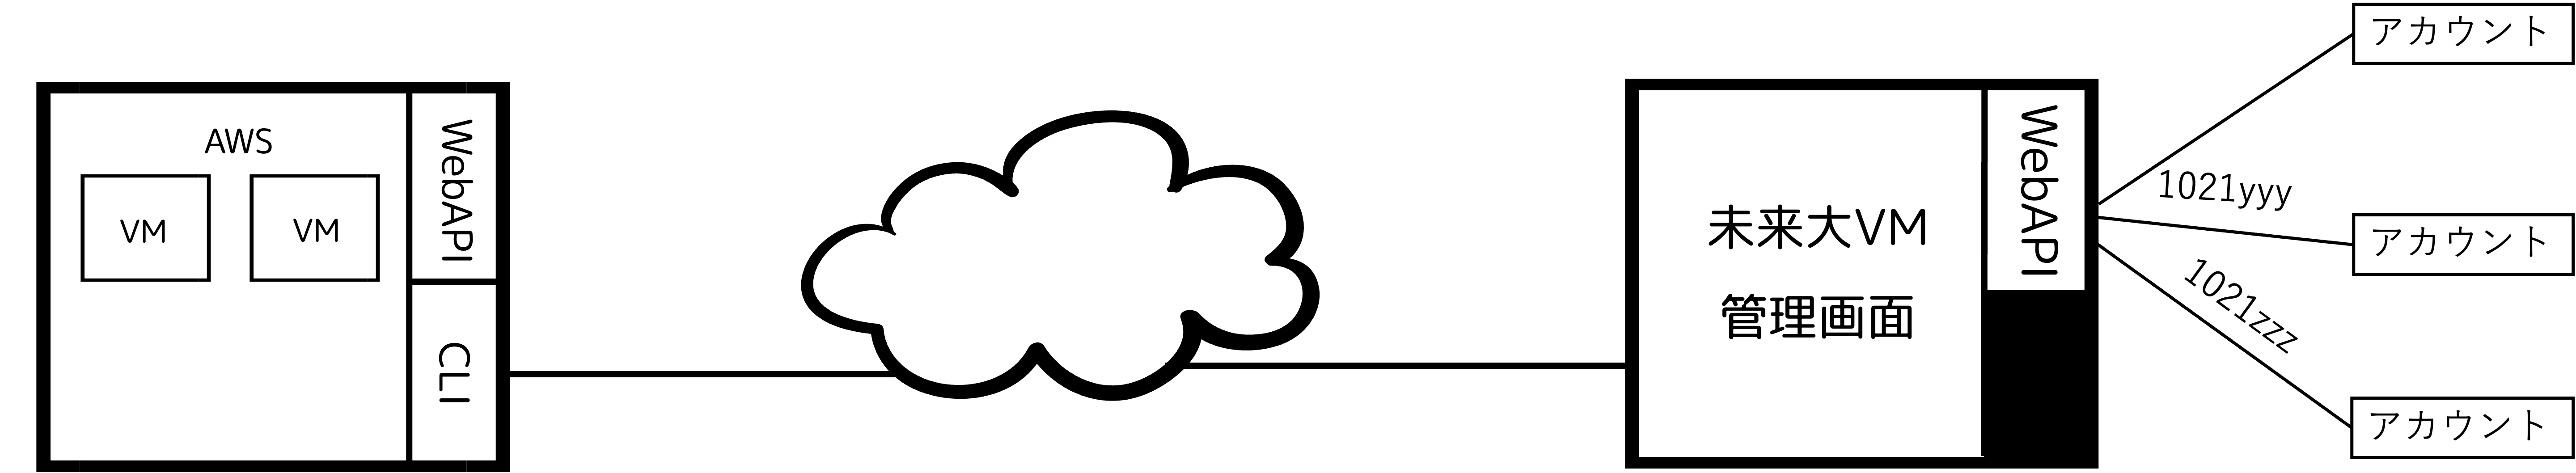
\includegraphics[width=1\linewidth,height=2cm]{./images/cloud.png}
	\caption{未来大クラウドシステムの構造}
	\label{fig:cloud}
\end{figure}



\section{提案}


本研究は,未来大クラウドシステムをスクレイピングによって活用し,未来大クラウドシステムのWebAPIを自動で操作することにより,
IaC対応化させることを提案する.
スクレイピングとは,WEBページ上のHTMLやCSSに存在するタグやデータ構造を解析し,構造化されているデータをプレーンなデータへと抽出し変換する技術である.
スクレイピングは,プログラムを使用して行われ,目的のWebページのHTMLデータを解析し,特定の情報をユーザからのリクエストに応じて自動的に取り出すことを可能にする.
ログイン認証が必要なページや,フォーム入力が必要な場合にも,スクレイピング技術は有効であり,ヘッドレスブラウザや専用のライブラリを使用し,自動的にフォームを入力,ログインプロセスを完了できる.

スクレイピングによって,未来大クラウドシステムのWebAPIを操作することにより,
学生アカウントごとのクラウドシステム管理を実現する
仮想マシンのコードを用いた管理と,コードの配布によるマシン環境の再現が可能となることで,
従来の演習用仮想マシンの準備と比べ,大幅な時間短縮を期待できる.


本研究では,IaCフレームワークにおけるデファクトスタンダードである,Terraformを利用する。
Terraformは,Amazon Web Services(以降,AWS)や
Microsoft Azure,Google Cloud Platformなどのクラウドプロバイダに対応しているため,
Terraformのコードを学習することで多くのプロバイダを同様のコマンドで管理できる.


\begin{figure}[h]
	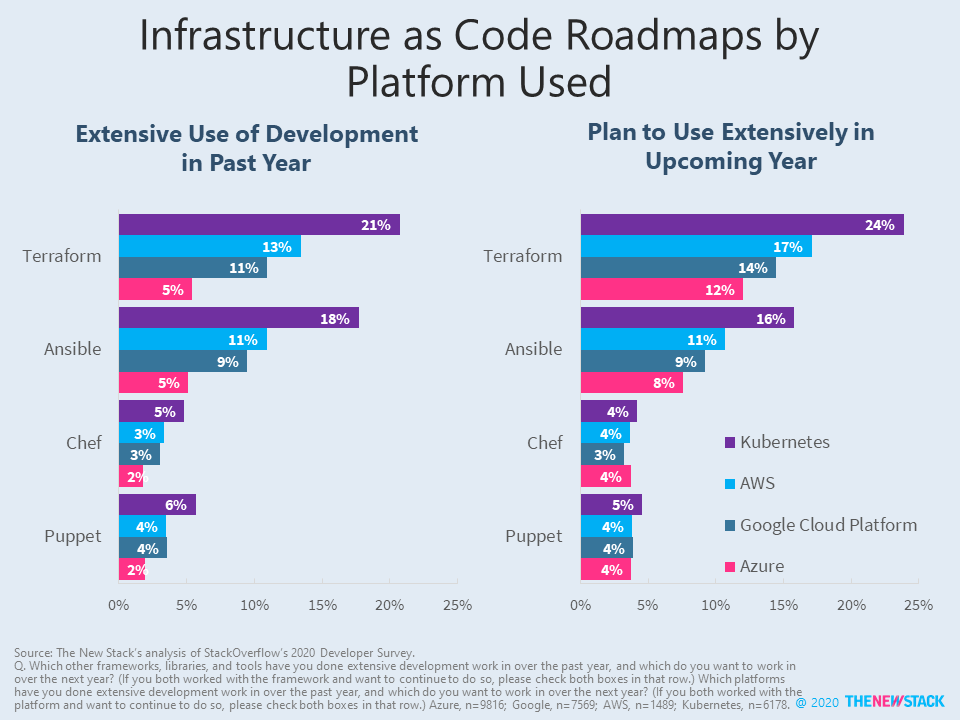
\includegraphics[width=1\linewidth]{./images/terraform.png}
	\caption{2020年のIaCプラットフォームの利用率比較\cite{THENEWSTACK}}
	\label{fig:terraform}
\end{figure}

Terraformは,プロビジョニング機能を備えている.プロビジョニング機能とは仮想マシンの作成・起動時に,仮想マシンの環境設定やプログラムの自動実行を行う機能である.
Terraformでは仮想マシン作成・起動後にマシンに対してSSH接続を行いプロビジョニング機能を実現している.

Terraform Custom Framework Providerという,新規にクラウドシステムをTerraformに対応させるプログラムが公開されている.
Terraform Custom Framework Providerは対応させたいクラウドシステムに合わせて書き換えることでTerraform対応を実現する.


本研究では,未来大クラウドシステム用のTerraform Custom Framework Providerを用意し,Terraform に対応させることで仮想マシンを管理する手法を確立する.
Terraformに対応させるために,クラウドシステムを直接操作するAPI使わず,
スクレイピングを活用し,未来大クラウドシステムのWebAPIを自動で操作することにより,未来大クラウドシステムの操作を実現する.


\begin{figure}[h]
	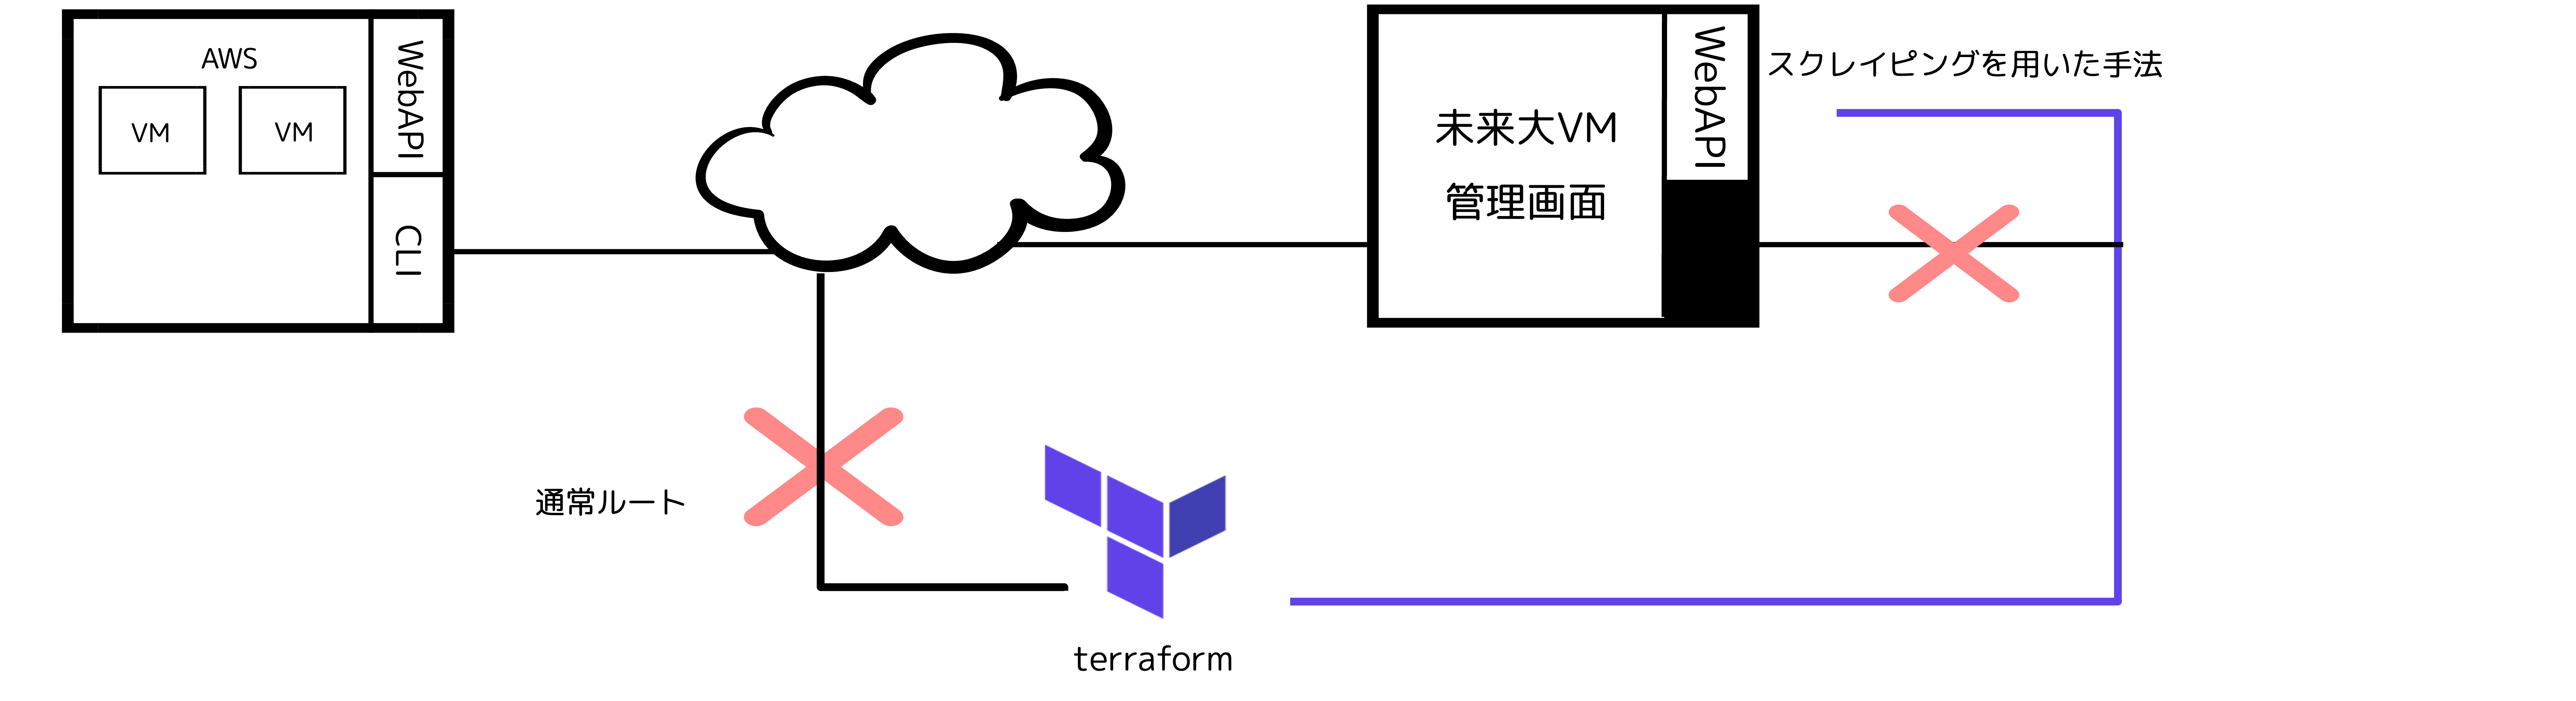
\includegraphics[width=1\linewidth]{./images/scraping.png}
	\caption{スクレイピングによる未来大クラウドシステムの管理}
	\label{fig:scraping}
\end{figure}








\section{実装}



本実装では,Terraformを用いてクラウドシステムを操作する際,仮想マシンの設定を記述したファイルを用意する.
未来大クラウドシステムを管理する際には、アカウント認証用のアカウント名,パスワード,演習環境の選択,管理するマシン名,マシンのスペック,マシンを停止させるかを記載する設計とする.


\begin{figure}[h]
	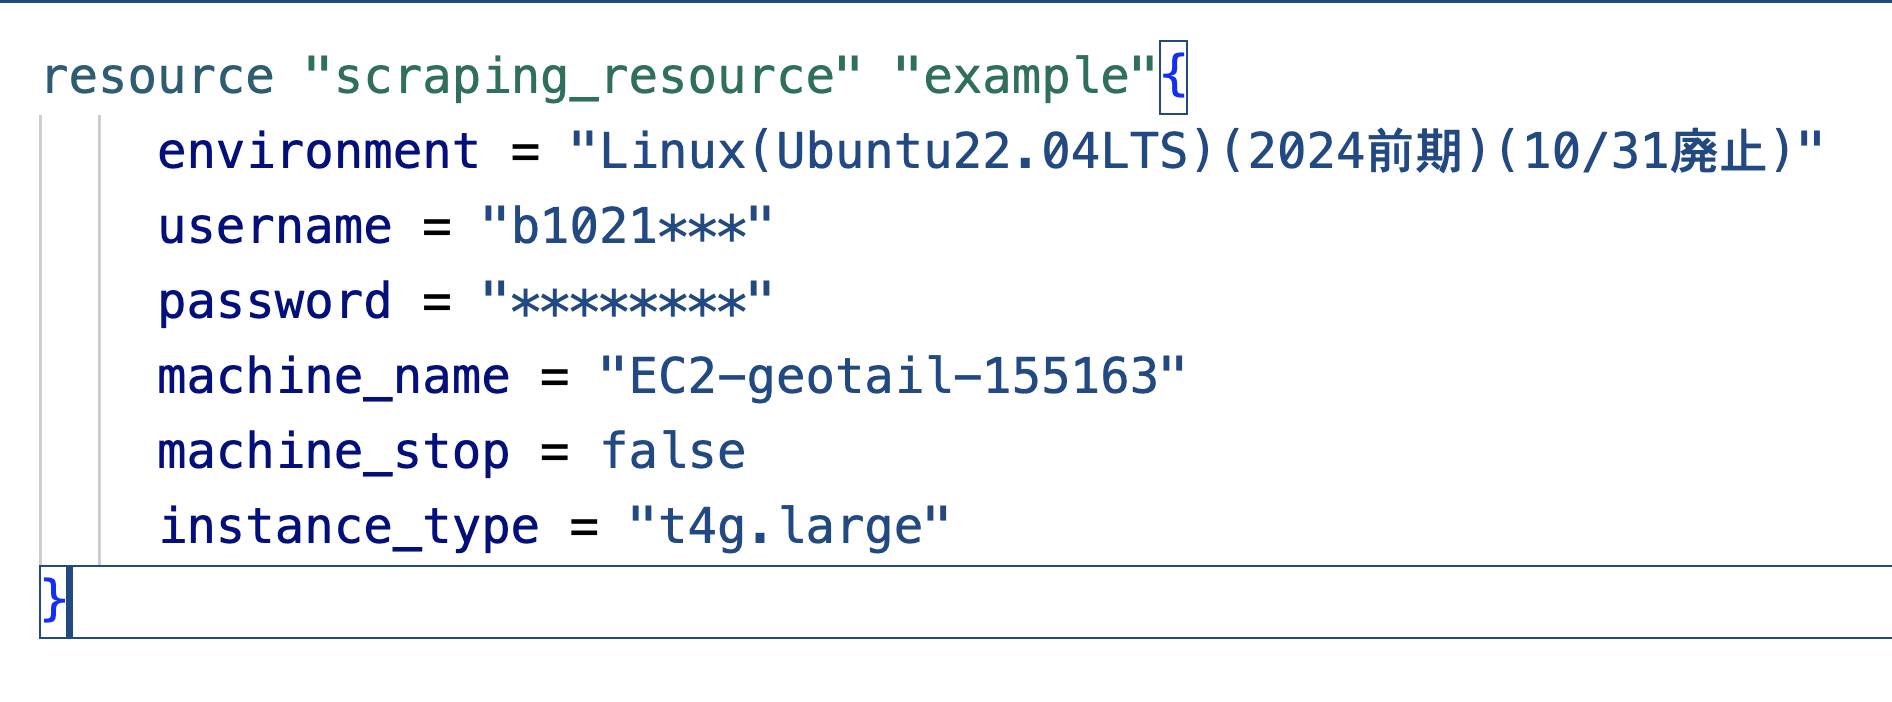
\includegraphics[width=1\linewidth]{./images/machine.png}
	\caption{設定ファイルの記述}
  \label{fig:machien}
\end{figure}


スクレイピングを用いて未来大クラウドシステムにアクセスすると,最初にユーザ認証画面へと遷移する.
ユーザー情報とパスワードをフォームに自動入力し,ボタンクリックを行うことで環境選択画面に遷移する.
環境選択では,年度や時期,受講している講義ごとに異なる環境を選択することが可能である.
設定ファイルで指定された環境選択と合致する文字列をドロップダウンから選択したのち,仮想マシン管理画面へ遷移する.
仮想マシン管理画面では,作成,起動,停止,削除の機能がある.
さらに,仮想マシンの作成,起動時では,仮想マシンのスペックを変更することが可能である.
設定ファイルでマシン名を指定せずに,Terraformの仮想マシン起動コマンドであるterraform applyを実行された時に,マシンの新規作成を行う設計とする.
設定ファイルでマシン名を指定し,terraform applyを行うことで,停止中の仮想マシンを起動できるよう設計する.作成,起動処理時に設定ファイルに記載されたマシンスペックに合致したものを選択する.

プロビジョニング機能を用いる際,仮想マシンのパスワードやIPアドレス,秘密鍵が必要となる.パスワードやIPアドレスはスクレイピングによって,
HTMLから自動抽出する機能を実装する.秘密鍵はWebAPIをスクレイピングして自動でダウンロードし,ダウンロード先の絶対パスを返す機能を実装する.


設定ファイルにて,仮想マシンの停止を要求するように記述し,terraform applyを行うことでWebAPIの停止ボタンを操作することで仮想マシンの停止が行われるよう実装する.
また,Terraformの仮想マシン削除コマンドであるterraform destroyを実行することによりWebAPIの削除ボタンを操作し,仮想マシンの削除機能を実現する.


本研究では,スクレイピングを行う処理をクラウドコンピュータ上で行う.クラウドコンピュータ上で行うことにより,手間となる関連モジュールのインストール工程
がなくなり、Terraformを実行する環境に左右されにくくなる.



\section{評価手法}

本システムの有用性を確認するために,
評価項目として定量的評価と定性的評価による測定を検討している.
定量的評価では,システムの使用における実行時間,システムそのもののレスポンス時間や安定性などのパフォーマンスメトリクスを測定する.
従来の講義準備にかかる時間と比較することで評価する.
定性的評価では,
未来大の2024年度後期の情報科学演習講義である並列分散処理の受講生を被験者として評価実験を行い,
アンケートを通じて被験者の使用感や満足度や要望,システムに対する意見を収集する.



\section{進捗と計画}

進捗状況として,スクレイピングを用いてTerraformによる未来大クラウドシステムの管理機能を実装した.
システムを使用するにあたり,
関連モジュールをインストールする手間を省くために,
クラウドコンピューティング上で実行,
実行環境に依存しないシステムの構築を目指している.
今後の計画として,クラウドコンピューティング上での実装が終わった後,実際に未来大の学生に使用してもらい,フィードバックを元に機能改善を目指す.


\section{結言}

本研究では,独自の管理インターフェースを持つ未来大クラウドシステムのIaC対応により,演習講義における統一環境準備の効率化を目指す.
クラウドシステムを直接管理することが困難なインターフェースのため,スクレイピングを用いて管理を行う.
今後の計画として,実行者のPC環境に依存しないように実装し,評価実験を行いたい.


\section{情報システムコースにおける本研究の位置づけ}

本研究では,スクレイピングにより学内クラウドシステムをIaCに対応させることによって,演習講義に用いる統一環境準備の効率化を目標としている.これは,未来大での演習講義を情報システムによって支援するものであり,効率性と信頼性を考慮した情報システムの実現と言える.
今後,実装したシステムを評価実験を行うことで,カリキュラムポリシーの結果の評価を通じて,新しい方法論や学問領域を切り拓く能力を育むことに繋がる.

\begin{thebibliography}{99}
	\bibitem{byod}
	大学ICT推進協議会: ICT利活用調査部会, "BYOD を活用した教育改善に関する調査研究 結果報告書", AXIES 大学ICT推進協議会.[Online]. Available from : \url{https://axies.jp/report/ict_survey/2016survey/}. Accessed: 2024-10-25.

	\bibitem{oosakadai}
	大阪大学, "大阪大学キャンパスクラウドサービス", 大阪大学. [Online]. Available from: \url{https://ccc.osaka-u.ac.jp/hosting/}. Accessed: 2024-10-21.
	\bibitem{O'Reilly Media}
	K. Morris: "Infrastructure as Code", O'Reilly Media, 2016.
	\bibitem{InformationSystem}
	Michele Chiari, Bin Xiang, Sergio Canzoneri, Galia Novakova Nedeltcheva, Elisabetta Di Nitto, Lorenzo Blasi, Debora Benedetto, Laurentiu Niculut, Igor Škof : "DOML: A new modeling approach to Infrastructure-as-Code", Information Systems, Volume 125, November 2024. 
	\bibitem{THENEWSTACK}
	B. Cameron Gain: "Terraform 1.0 Reflects What HashiCorp Has Learned About Infrastructure-as-Code", THENEWSTACK, [Online]. Available from: \url{https://thenewstack.io/terraform1-0-reflects-what-hashicorp-has-learned-about-infrastructure-as-code/?utm_referrer=https%3A%2F%2Fwww.google.com%2F/}. Accessed: 2024-10-22.
	%\bibitem{selenium}
	%SeleniumHQ, "Selenium Documentation", Selenium, 2023. [Online]. Available from: \url{https://www.selenium.dev/documentation/en/}. Accessed: 2023-10-25.
\end{thebibliography}
\end{document}
%
%
% EOF